\hypertarget{fk-methods}{%
\section{Methods}\label{fk-methods}}

\hypertarget{thermodynamics-of-the-lrfk-model}{%
\subsection{Thermodynamics of the LRFK Model}\label{thermodynamics-of-the-lrfk-model}}

The results for the phase diagram were obtained with a classical Markov Chain Monte Carlo (MCMC) method which we discuss in the following. It allows us to solve our long-range FK model efficiently, yielding unbiased estimates of thermal expectation values and linking it to disorder physics in a translationally invariant setting.

Since the spin configurations are classical, the Hamiltonian can be split into a classical spin part \(H_s\) and an operator valued part \(H_c\).

\[\begin{aligned}
H_s& = - \frac{U}{2}S_i + \sum_{i, j}^{N} J_{ij} S_i S_j \\
H_c& = \sum_i U S_i c^\dagger_{i}c_{i} -t(c^\dagger_{i}c_{i+1} + c^\dagger_{i+1}c_{i}) \end{aligned}\]

The partition function can then be written as a sum over spin configurations, \(\vec{S} = (S_0, S_1...S_{N-1})\):

\[\begin{aligned}
\mathcal{Z} = \mathrm{Tr} e^{-\beta H}= \sum_{\vec{S}} e^{-\beta H_s} \mathrm{Tr}_c e^{-\beta H_c} .\end{aligned}\]

The contribution of \(H_c\) to the grand canonical partition function can be obtained by performing the sum over eigenstate occupation numbers giving \(-\beta F_c[\vec{S}] = \sum_k \ln{(1 + e^{- \beta \epsilon_k})}\) where \({\epsilon_k[\vec{S}]}\) are the eigenvalues of the matrix representation of \(H_c\) determined through exact diagonalisation. This gives a partition function containing a classical energy which corresponds to the long-range interaction of the spins, and a free energy which corresponds to the quantum subsystem. \[\begin{aligned}
\mathcal{Z} = \sum_{\vec{S}} e^{-\beta H_S[\vec{S}] - \beta F_c[\vec{S}]} = \sum_{\vec{S}} e^{-\beta E[\vec{S}]}\end{aligned}\]

\hypertarget{markov-chain-monte-carlo-and-emergent-disorder}{%
\subsection{Markov Chain Monte Carlo and Emergent Disorder}\label{markov-chain-monte-carlo-and-emergent-disorder}}

Classical MCMC defines a weighted random walk over the spin states \((\vec{S}_0, \vec{S}_1, \vec{S}_2, ...)\), such that the likelihood of visiting a particular state converges to its Boltzmann probability \(p(\vec{S}) = \mathcal{Z}^{-1} e^{-\beta E}\). Hence, any observable can be estimated as a mean over the states visited by the walk~\autocite{binderGuidePracticalWork1988,kerteszAdvancesComputerSimulation1998,wolffMonteCarloErrors2004}, \[\begin{aligned}
\label{eq:thermal_expectation}
\langle O \rangle & = \sum_{\vec{S}} p(\vec{S}) \langle O \rangle_{\vec{S}}\\
                  & = \sum_{i = 0}^{M} \langle O\rangle_{\vec{S}_i} \pm \mathcal{O}(\tfrac{1}{\sqrt{M}})
\end{aligned}\] where the former sum runs over the entire state space while the later runs over all the state visited by a particular MCMC run.

\[\begin{aligned}
\langle O \rangle_{\vec{S}}& = \sum_{\nu} n_F(\epsilon_{\nu}) \langle O \rangle{\nu}
\end{aligned}\]

Where \(\nu\) runs over the eigenstates of \(H_c\) for a particular spin configuration and \(n_F(\epsilon) = \left(e^{-\beta\epsilon} + 1\right)^{-1}\) is the Fermi function.

The choice of the transition function for MCMC is under-determined as one only needs to satisfy a set of balance conditions for which there are many solutions~\autocite{kellyReversibilityStochasticNetworks1981}. Here, we incorporate a modification to the standard Metropolis-Hastings algorithm~\autocite{hastingsMonteCarloSampling1970} gleaned from Krauth~\autocite{krauthIntroductionMonteCarlo1998}. Let us first recall the standard algorithm which decomposes the transition probability into \(\mathcal{T}(a \to b) = p(a \to b)\mathcal{A}(a \to b)\). Here, \(p\) is the proposal distribution that we can directly sample from while \(\mathcal{A}\) is the acceptance probability. The standard Metropolis-Hastings choice is \[\mathcal{A}(a \to b) = \min\left(1, \frac{p(b\to a)}{p(a\to b)} e^{-\beta \Delta E}\right)\;,\] with \(\Delta E = E_b - E_a\). The walk then proceeds by sampling a state \(b\) from \(p\) and moving to \(b\) with probability \(\mathcal{A}(a \to b)\). The latter operation is typically implemented by performing a transition if a uniform random sample from the unit interval is less than \(\mathcal{A}(a \to b)\) and otherwise repeating the current state as the next step in the random walk. The proposal distribution is often symmetric so does not appear in \(\mathcal{A}\). Here, we flip a small number of sites in \(b\) at random to generate proposals, which is indeed symmetric.

In our computations~\autocite{hodsonMCMCFKModel2021} we employ a modification of the algorithm which is based on the observation that the free energy of the {FK} system is composed of a classical part which is much quicker to compute than the quantum part. Hence, we can obtain a computational speedup by first considering the value of the classical energy difference \(\Delta H_s\) and rejecting the transition if the former is too high. We only compute the quantum energy difference \(\Delta F_c\) if the transition is accepted. We then perform a second rejection sampling step based upon it. This corresponds to two nested comparisons with the majority of the work only occurring if the first test passes and has the acceptance function \[\mathcal{A}(a \to b) = \min\left(1, e^{-\beta \Delta H_s}\right)\min\left(1, e^{-\beta \Delta F_c}\right)\;.\]

For the model parameters used in Fig.~{[}1{]}, we find that with our new scheme the matrix diagonalisation is skipped around 30\% of the time at \(T = 2.5\) and up to 80\% at \(T = 1.5\). We observe that for \(N = 50\), the matrix diagonalisation, if it occurs, occupies around 60\% of the total computation time for a single step. This rises to 90\% at N = 300 and further increases for larger N. We therefore get the greatest speedup for large system sizes at low temperature where many prospective transitions are rejected at the classical stage and the matrix computation takes up the greatest fraction of the total computation time. The upshot is that we find a speedup of up to a factor of 10 at the cost of very little extra algorithmic complexity.

Our two-step method should be distinguished from the more common method for speeding up MCMC which is to add asymmetry to the proposal distribution to make it as similar as possible to \(\min\left(1, e^{-\beta \Delta E}\right)\). This reduces the number of rejected states, which brings the algorithm closer in efficiency to a direct sampling method. However it comes at the expense of requiring a way to directly sample from this complex distribution, a problem which MCMC was employed to solve in the first place. For example, recent work trains restricted Boltzmann machines (RBMs) to generate samples for the proposal distribution of the FK model~\autocite{huangAcceleratedMonteCarlo2017}. The RBMs are chosen as a parametrisation of the proposal distribution that can be efficiently sampled from while offering sufficient flexibility that they can be adjusted to match the target distribution. Our proposed method is considerably simpler and does not require training while still reaping some of the benefits of reduced computation.

\hypertarget{application-to-the-fk-model}{%
\subsection{Application to the FK Model}\label{application-to-the-fk-model}}

We will work in the grand canonical ensemble of fixed temperature, chemical potential and volume.

Since the spin configurations are classical, the Hamiltonian can be split into a classical spin part \(H_s\) and an operator valued part \(H_c\). \[\begin{aligned}
H_s& = - \frac{U}{2}S_i + \sum_{i, j}^{N} J_{ij} S_i S_j \\
H_c& = \sum_i U S_i c^\dagger_{i}c_{i} -t(c^\dagger_{i}c_{i+1} + c^\dagger_{i+1}c_{i}) 
\end{aligned}\] The partition function can then be written as a sum over spin configurations, \(\vec{S} = (S_0, S_1...S_{N-1})\): \[\begin{aligned}
\mathcal{Z} = \mathrm{Tr} e^{-\beta H}= \sum_{\vec{S}} e^{-\beta H_s} \mathrm{Tr}_c e^{-\beta H_c} .
\end{aligned}
\] The contribution of \(H_c\) to the grand canonical partition function can be obtained by performing the sum over eigenstate occupation numbers giving \(-\beta F_c[\vec{S}] = \sum_k \ln{(1 + e^{- \beta \epsilon_k})}\) where \({\epsilon_k[\vec{S}]}\) are the eigenvalues of the matrix representation of \(H_c\) determined through exact diagonalisation. This gives a partition function containing a classical energy which corresponds to the long-range interaction of the spins, and a free energy which corresponds to the quantum subsystem. \[\begin{aligned}
\mathcal{Z} = \sum_{\vec{S}} e^{-\beta H_S[\vec{S}] - \beta F_c[\vec{S}]} = \sum_{\vec{S}} e^{-\beta E[\vec{S}]}
\end{aligned}\]

\hypertarget{two-step-trick}{%
\subsection{Two Step Trick}\label{two-step-trick}}

Here, we incorporate a modification to the standard Metropolis-Hastings algorithm~\autocite{hastingsMonteCarloSampling1970} gleaned from Krauth~\autocite{krauthIntroductionMonteCarlo1998}.

In our computations~\autocite{hodsonMCMCFKModel2021} we employ a modification of the algorithm which is based on the observation that the free energy of the FK system is composed of a classical part which is much quicker to compute than the quantum part. Hence, we can obtain a computational speedup by first considering the value of the classical energy difference \(\Delta H_s\) and rejecting the transition if the former is too high. We only compute the quantum energy difference \(\Delta F_c\) if the transition is accepted. We then perform a second rejection sampling step based upon it. This corresponds to two nested comparisons with the majority of the work only occurring if the first test passes and has the acceptance function \[\mathcal{A}(a \to b) = \min\left(1, e^{-\beta \Delta H_s}\right)\min\left(1, e^{-\beta \Delta F_c}\right)\;.\]

For the model parameters \(U=2/5, T = 1.5 / 2.5, J = 5,\;\alpha = 1.25\), we find that with our new scheme the matrix diagonalisation is skipped around 30\% of the time at \(T = 2.5\) and up to 80\% at \(T = 1.5\). We observe that for \(N = 50\), the matrix diagonalisation, if it occurs, occupies around 60\% of the total computation time for a single step. This rises to 90\% at N = 300 and further increases for larger N. We therefore get the greatest speedup for large system sizes at low temperature where many prospective transitions are rejected at the classical stage and the matrix computation takes up the greatest fraction of the total computation time. The upshot is that we find a speedup of up to a factor of 10 at the cost of very little extra algorithmic complexity.

Our two-step method should be distinguished from the more common method for speeding up MCMC which is to add asymmetry to the proposal distribution to make it as similar as possible to \(\min\left(1, e^{-\beta \Delta E}\right)\). This reduces the number of rejected states, which brings the algorithm closer in efficiency to a direct sampling method. However it comes at the expense of requiring a way to directly sample from this complex distribution, a problem which MCMC was employed to solve in the first place. For example, recent work trains restricted Boltzmann machines (RBMs) to generate samples for the proposal distribution of the FK model~\autocite{huangAcceleratedMonteCarlo2017}. The RBMs are chosen as a parametrisation of the proposal distribution that can be efficiently sampled from while offering sufficient flexibility that they can be adjusted to match the target distribution. Our proposed method is considerably simpler and does not require training while still reaping some of the benefits of reduced computation.

\hypertarget{scaling}{%
\subsection{Scaling}\label{scaling}}

In order to reduce the effects of the boundary conditions and the finite size of the system we redefine and normalise the coupling matrix to have 0 derivative at its furthest extent rather than cutting off abruptly.

\[
\begin{aligned}
J'(x) &= \abs{\frac{L}{\pi}\sin \frac{\pi x}{L}}^{-\alpha} \\
J(x) &= \frac{J_0 J'(x)}{\sum_y J'(y)}
\end{aligned}\] \% The scaling ensures that, in the ordered phase, the overall potential felt by each site due to the rest of the system is independent of system size.

\hypertarget{binder-cumulants}{%
\subsection{Binder Cumulants}\label{binder-cumulants}}

The Binder cumulant is defined as: \[U_B = 1 - \frac{\tex{\mu_4}}{3\tex{\mu_2}^2}\] \% where \[\mu_n = \tex{(m - \tex{m})^n}\] \% are the central moments of the order parameter m: \[m = \sum_i (-1)^i (2n_i - 1) / N\] \% The Binder cumulant evaluated against temperature can be used as a diagnostic for the existence of a phase transition. If multiple such curves are plotted for different system sizes, a crossing indicates the location of a critical point~\autocite{binderFiniteSizeScaling1981,musialMonteCarloSimulations2002}.

\hypertarget{diagnostics-of-localisation}{%
\subsection{Diagnostics of Localisation}\label{diagnostics-of-localisation}}

\hypertarget{inverse-participation-ratio}{%
\subsubsection{Inverse Participation Ratio}\label{inverse-participation-ratio}}

The inverse participation ratio is defined for a normalised wave function \(\psi_i = \psi(x_i), \sum_i \abs{\psi_i}^2 = 1\) as its fourth moment~\autocite{kramerLocalizationTheoryExperiment1993}: \[
P^{-1} = \sum_i \abs{\psi_i}^4
\] \% It acts as a measure of the portion of space occupied by the wave function. For localised states it will be independent of system size while for plane wave states in d dimensions \$P = L\^{}d \$. States may also be intermediate between localised and extended, described by their fractal dimensionality \(d > d* > 0\): \[
P(L) \goeslike L^{d*} 
\] \% For extended states \(d* = 0\) while for localised ones \(d* = 0\). In this work we take use an energy resolved IPR~\autocite{andersonAbsenceDiffusionCertain1958}: \[
DOS(\omega) = \sum_n \delta(\omega - \epsilon_n)
IPR(\omega) = DOS(\omega)^{-1} \sum_{n,i} \delta(\omega - \epsilon_n) \abs{\psi_{n,i}}^4
\] Where \(\psi_{n,i}\) is the wavefunction corresponding to the energy \(\epsilon_n\) at the ith site. In practice we bin the energies and IPRs into a fine energy grid and use Lorentzian smoothing if necessary.

\begin{figure}
\hypertarget{fig:raw}{%
\centering
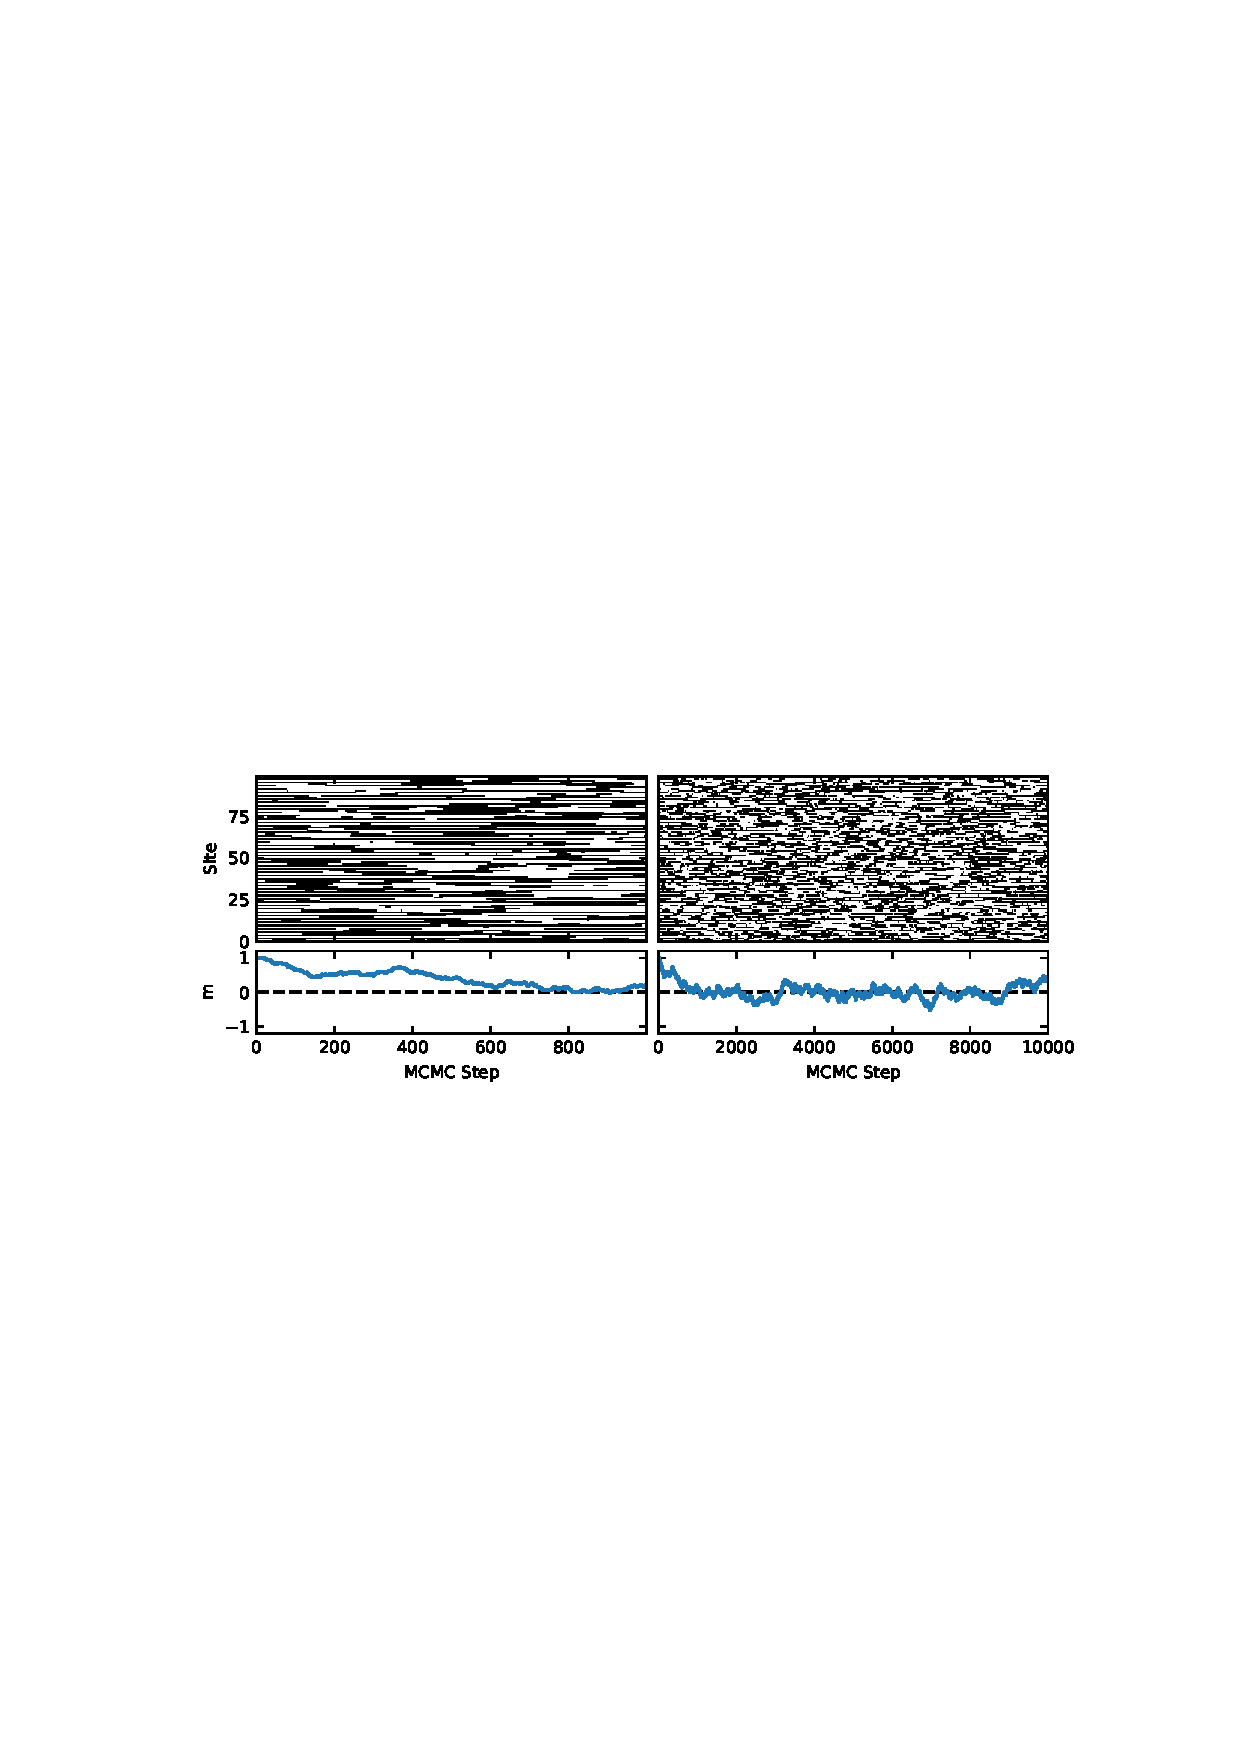
\includegraphics{figs/lsr/raw_steps_single_flip.pdf}
\caption{An MCMC walk starting from the staggered charge density wave ground state for a system with \(N = 100\) sites and 10,000 MCMC steps. In this simulation only a single spin can be flipped per step according to the Metropolis-Hastings Algorithm. The staggered magnetisation \(m = N^{-1} \sum_i (-1)^i \; S_i\) order parameter is plotted below. At this temperature the thermal average of m is zero, while the initial state has m = 1. We see that it takes about 1000 steps for the system to converge, after which it moves about the m = 0 average with a finite auto-correlation time. \(t = 1, \alpha = 1.25, T = 3, J = U = 5\) \protect\hypertarget{fig:raw}{}{{[}fig:raw{]}}}\label{fig:raw}
}
\end{figure}

{MCMC} sidesteps these issues by defining a random walk that focuses on the states with the greatest Boltzmann weight. At low temperatures this means we need only visit a few low energy states to make good estimates while at high temperatures the weights become uniform so a small number of samples distributed across the state space suffice. However we will see that the method is not without difficulties of its own.

\begin{figure}
\hypertarget{fig:single}{%
\centering
\includegraphics{figs/lsr/single.pdf}
\caption{Two MCMC chains starting from the same initial state for a system with \(N = 90\) sites and 1000 MCMC steps. In this simulation the MCMC step is defined differently: an attempt is made to flip n spins, where n is drawn from Uniform(1,N). This is repeated \(N^2/100\) times for each step. This trades off computation time for storage space, as it makes the samples less correlated, giving smaller statistical error for a given number of stored samples. These simulations therefore have the potential to necessitate \(N^2/100\) matrix diagonalisations for every MCMC sample, though this can be cut down with caching and other tricks. \(t = 1, \alpha = 1.25, T = 2.2, J = U = 5\) \protect\hypertarget{fig:single}{}{{[}fig:single{]}}}\label{fig:single}
}
\end{figure}

In implementation {MCMC} can be boiled down to choosing a transition function \(\mathcal{T}(\s_{t} \rightarrow \s_t+1)\) where \(\s\) are vectors representing classical spin configurations. We start in some initial state \(\s_0\) and then repeatedly jump to new states according to the probabilities given by \(\mathcal{T}\). This defines a set of random walks \(\{\s_0\ldots \s_i\ldots \s_N\}\). Fig.~\protect\hyperlink{fig:single}{2} shows this in practice: we have a (rather small) ensemble of \(M = 2\) walkers starting at the same point in state space and then spreading outwards by flipping spins along the way.

In pseudo-code one could write the MCMC simulation for a single walker as:

``\,'python current\_state = initial\_state

for i in range(N\_steps): new\_state = sample\_T(current\_state) states{[}i{]} = current\_state ``\,'

Where the \texttt{sample\_T} function here produces a state with probability determined by the \texttt{current\_state} and the transition function \(\mathcal{T}\).

If we ran many such walkers in parallel we could then approximate the distribution \(p_t(\s; \s_0)\) which tells us where the walkers are likely to be after they've evolved for \(t\) steps from an initial state \(\s_0\). We need to carefully choose \(\mathcal{T}\) such that after a large number of steps \(k\) (the convergence time) the probability \(p_t(\s;\s_0)\) approaches the thermal distribution \(P(\s; \beta) = \mathcal{Z}^{-1} e^{-\beta F(\s)}\). This turns out to be quite easy to achieve using the Metropolis-Hasting algorithm.

\hypertarget{convergence-time}{%
\subsection{Convergence Time}\label{convergence-time}}

Considering \(p(\s)\) as a vector \(\vec{p}\) whose jth entry is the probability of the jth state \(p_j = p(\s_j)\), and writing \(\mathcal{T}\) as the matrix with entries \(T_{ij} = \mathcal{T}(\s_j \rightarrow \s_i)\) we can write the update rule for the ensemble probability as: \[\vec{p}_{t+1} = \mathcal{T} \vec{p}_t \implies \vec{p}_{t} = \mathcal{T}^t \vec{p}_0\] where \(\vec{p}_0\) is vector which is one on the starting state and zero everywhere else. Since all states must transition to somewhere with probability one: \(\sum_i T_{ij} = 1\).

Matrices that satisfy this are called stochastic matrices exactly because they model these kinds of Markov processes. It can be shown that they have real eigenvalues, and ordering them by magnitude, that \(\lambda_0 = 1\) and \(0 < \lambda_{i\neq0} < 1\). Assuming \(\mathcal{T}\) has been chosen correctly, its single eigenvector with eigenvalue 1 will be the thermal distribution {[}\^{}3{]} so repeated application of the transition function eventually leads there, while memory of the initial conditions decays exponentially with a convergence time \(k\) determined by \(\lambda_1\). In practice this means that one throws away the data from the beginning of the random walk in order reduce the dependence on the initial conditions and be close enough to the target distribution.

\hypertarget{auto-correlation-time}{%
\subsection{Auto-correlation Time}\label{auto-correlation-time}}

\begin{figure}
\hypertarget{fig:m_autocorr}{%
\centering
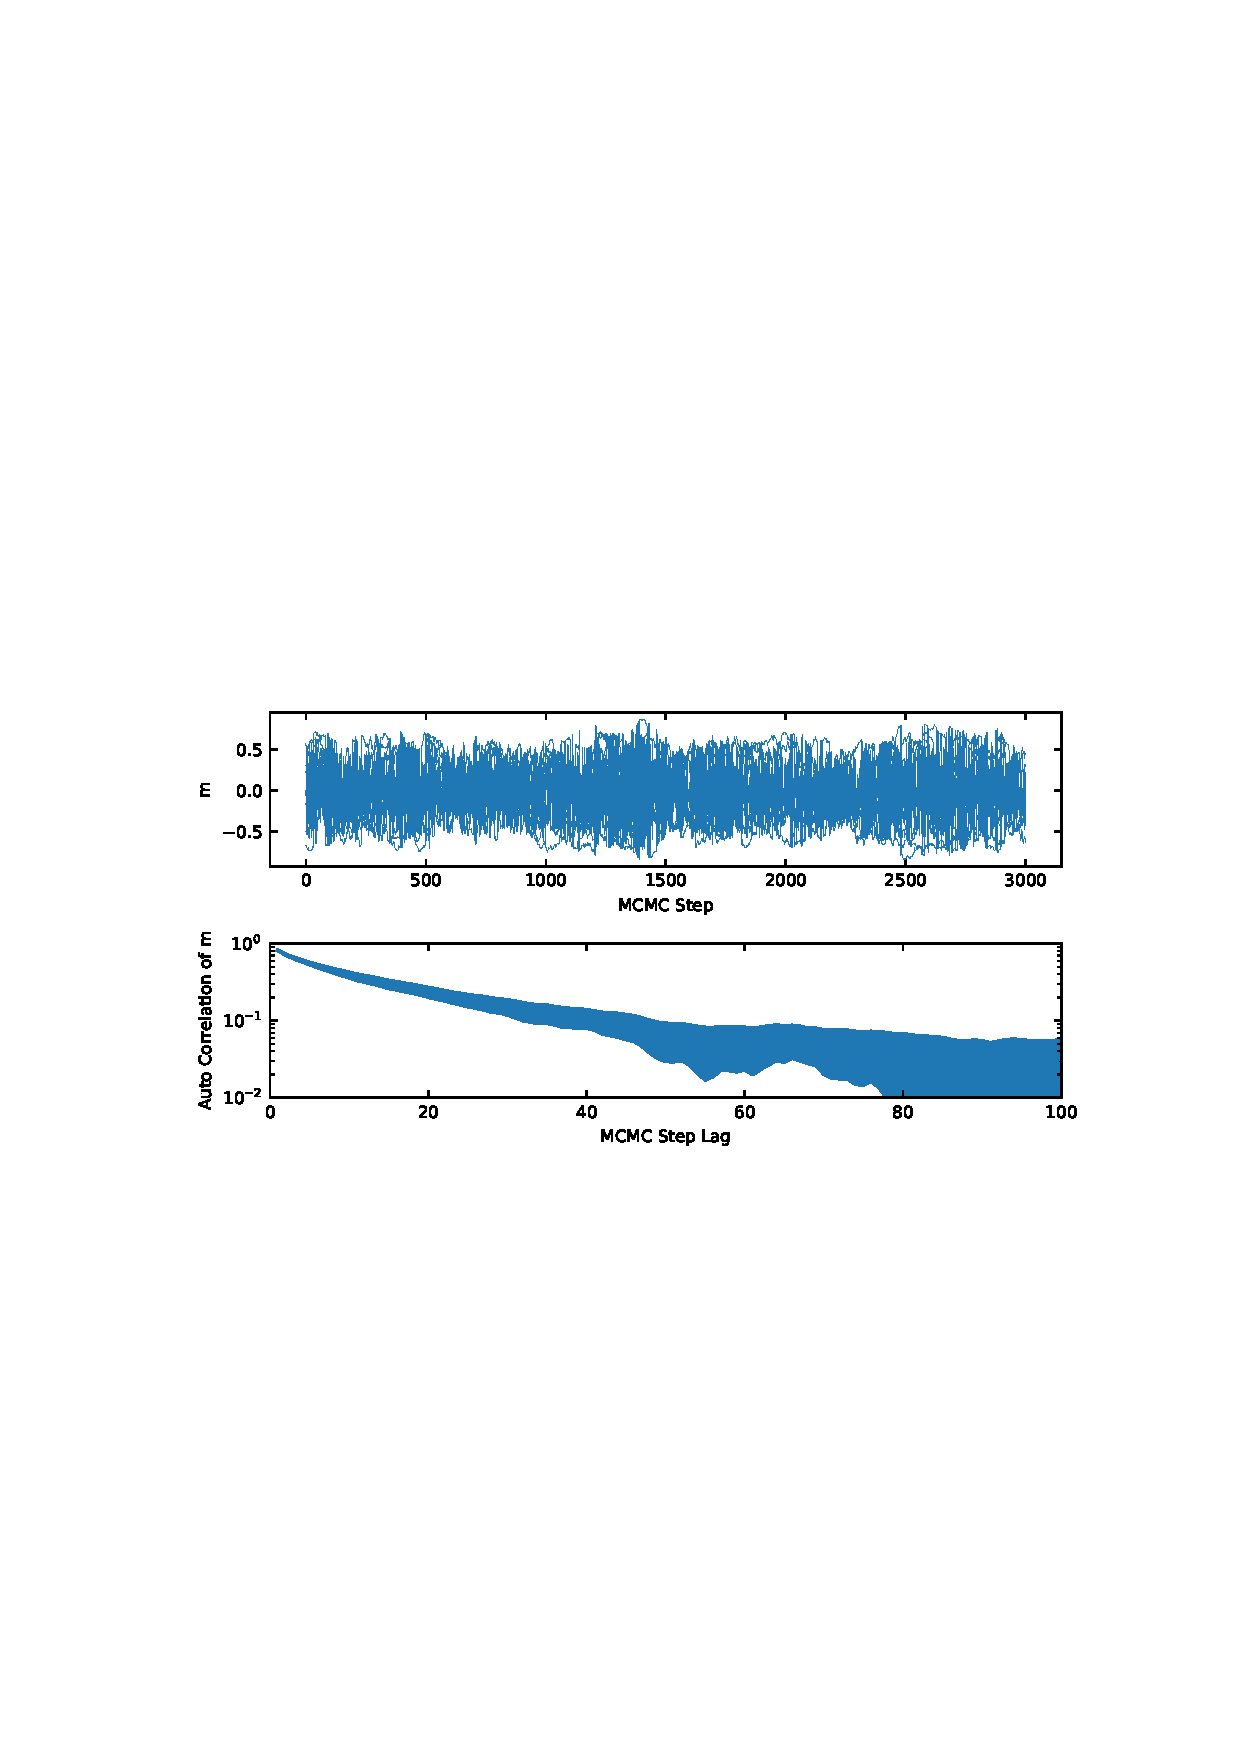
\includegraphics{figs/lsr/m_autocorr.png}
\caption{(Upper) 10 MCMC chains starting from the same initial state for a system with \(N = 150\) sites and 3000 MCMC steps. At each MCMC step, n spins are flipped where n is drawn from Uniform(1,N) and this is repeated \(N^2/100\) times. The simulations therefore have the potential to necessitate \(10*N^2\) matrix diagonalisations for each 100 MCMC steps. (Lower) The normalised auto-correlation \((\expval{m_i m_{i-j}} - \expval{m_i}\expval{m_i}) / Var(m_i))\) averaged over \(i\). It can be seen that even with each MCMC step already being composed of many individual flip attempts, the auto-correlation is still non negligible and must be taken into account in the statistics. \(t = 1, \alpha = 1.25, T = 2.2, J = U = 5\) \protect\hypertarget{fig:m_autocorr}{}{{[}fig:m\_autocorr{]}}}\label{fig:m_autocorr}
}
\end{figure}

At this stage one might think we're done. We can indeed draw independent samples from \(P(\s; \beta)\) by starting from some arbitrary initial state and doing \(k\) steps to arrive at a sample. However a key insight is that after the convergence time, every state generated is a sample from \(P(\s; \beta)\)! They are not, however, independent samples. In Fig.~\protect\hyperlink{fig:raw}{1} it is already clear that the samples of the order parameter m have some auto-correlation because only a few spins are flipped each step but even when the number of spins flipped per step is increased, Fig.~\protect\hyperlink{fig:m_autocorr}{3} shows that it can be an important effect near the phase transition. Let's define the auto-correlation time \(\tau(O)\) informally as the number of MCMC samples of some observable O that are statistically equal to one independent sample.~{[}\^{}4{]} The auto-correlation time is generally shorter than the convergence time so it therefore makes sense from an efficiency standpoint to run a single walker for many MCMC steps rather than to run a huge ensemble for \(k\) steps each.

Once the random walk has been carried out for many steps, the expectation values of \(O\) can be estimated from the MCMC samples \(\s_i\): \[\tex{O} = \sum_{i = 0}^{N} O(\s_i) + \mathcal{O}(\frac{1}{\sqrt{N}})\] The the samples are correlated so the N of them effectively contains less information than \(N\) independent samples would, in fact roughly \(N/\tau\) effective samples. As a consequence the variance is larger than the \(\qex{O^2} - \qex{O}^2\) form it would have if the estimates were uncorrelated. There are many methods in the literature for estimating the true variance of \(\qex{O}\) and deciding how many steps are needed but my approach has been to run a small number of parallel chains, which are independent, in order to estimate the statistical error produced. This is a slightly less computationally efficient because it requires throwing away those \(k\) steps generated before convergence multiple times but it is a conceptually simple workaround.

In summary, to do efficient simulations we want to reduce both the convergence time and the auto-correlation time as much as possible. In order to explain how, we need to introduce the Metropolis-Hasting (MH) algorithm and how it gives an explicit form for the transition function.
